\documentclass{article}
\usepackage{marginnote}
\usepackage{lipsum}
\usepackage[utf8]{inputenc}
\usepackage[T1]{fontenc}
\usepackage[spanish]{babel}
\usepackage[T1]{fontenc}
\usepackage{graphicx}
\usepackage{xcolor}
\usepackage{titlesec}
\usepackage{ragged2e}
\usepackage{tikz}
\usepackage{geometry}
\usepackage{adjustbox}
\geometry{a4paper, left=2cm, right=6cm, top=2.5cm, bottom=2.5cm} % Ajuste de márgenes
\usepackage{eso-pic}
\usepackage{fancyhdr}  % Paquete para encabezados y pies de página personalizados
\usepackage{fancybox}
\usepackage{fontspec}
\usepackage{eso-pic}
\setlength{\headheight}{77.79024pt} % Ajusta el valor según sea necesario
\setmainfont{Arial}
% Definición de colores personalizados
\definecolor{primary}{HTML}{483D8B}  % Color azul oscuro
\definecolor{secondary}{HTML}{8A2BE2}  % Color púrpura
\definecolor{highlight}{HTML}{0000FF}  % Color azul
\definecolor{positive}{HTML}{1E90FF}  % Color azul claro para positivos
\definecolor{neutral}{HTML}{9370DB}  % Color púrpura suave para neutrales
\definecolor{negative}{HTML}{8B0000}  % Color rojo oscuro para negativos


\AddToShipoutPictureBG*{
    {
        \hspace{16cm}
\includegraphics[width=6cm,keepaspectratio]{static/CosoAbajo.png} % Ajusta el tamaño y la ruta de la imagen
    }
}

\begin{document}
\vspace*{0.1em}
% Configuración del encabezado
\pagestyle{fancy}
\fancyhf{}  % Limpia encabezado y pie de página
\fancyhead[L]{\includegraphics[width=7cm]{static/logo.png}}  % Logo en la esquina superior izquierda
\renewcommand{\headrulewidth}{0pt}  % Quita la línea del encabezado
\vspace{2em}

% Título en la misma página
\begin{flushleft}
    \marginnote{\scriptsize \parbox{3cm}{\justify La IA aplicada al analisis de respuestas de las personas encuestadas te permite una comprension profunda y aporta claridad y profundidad en el diagnostico de los factores que influyen en la satisfaccion y el compromiso de tu equipo. facilitando una intervencion mas informada y efectiva,}}
    
    \begin{tikzpicture}[baseline=(A.base)]
        % Ovalo personalizado
        \node[draw, color=primary, thick, rounded corners=10pt, minimum width=4cm, minimum height=1.3cm, text centered] (A) 
            {\large \textbf{Informe diagnóstico}};
        % Línea que conecta el óvalo con la nota al margen
        \draw[thick, color=primary] (A.east) -- ++(10cm, 0);
    \end{tikzpicture}
\end{flushleft}
% Resumen y conclusión


\begin{flushleft}
\begin{minipage}[t]{0.9\textwidth}  % Ajusta el valor del 0.85 según lo necesites
\vspace{2em}
\normalsize\justifying{{{conclusion}}\\ }
\end{minipage}
\end{flushleft}


\begin{figure}[h!]
\begin{flushleft}
    \marginnote{\scriptsize \parbox{3cm}{\justify Las emociones seleccionadas para este análisis (Sorpresa, Tristeza, Desprecio, Miedo, Ira, Asco y Alegría) son fundamentales en la teoría psicológica y el análisis de sentimientos, ya que cubren un amplio espectro de respuestas emocionales humanas,  reconocidas, demostradas y clasificadas en diversas teorías del ámbito de la Psicología. En nuestro modelo nos hemos basado en autores tan reconocidos como Ekman(1992, 1999), Plutchik (1980, 2001) y Lazarus \& Lazarus (1996), entre otros.
    
    Lo que ves a continuación es un gráfico en el que, utilizando nuestros algoritmos de PLN (Procesamiento de Lenguaje Natural)., te mostramos las emociones predominantes en tus compañeros a partir del análisis de los textos que nos habéis entregado. }}
    \begin{tikzpicture}[baseline=(A.base)]
        % Ovalo personalizado
        \node[draw, color=primary, thick, rounded corners=10pt, minimum width=4cm, minimum height=1.3cm, text centered] (A) 
            {\large \textbf{Análisis de Términos Generales}};
        % Línea que conecta el óvalo con la nota al margen
        \draw[thick, color=primary] (A.east) -- ++(7.5cm, 0);
    \end{tikzpicture}
\end{flushleft}
    \centering
    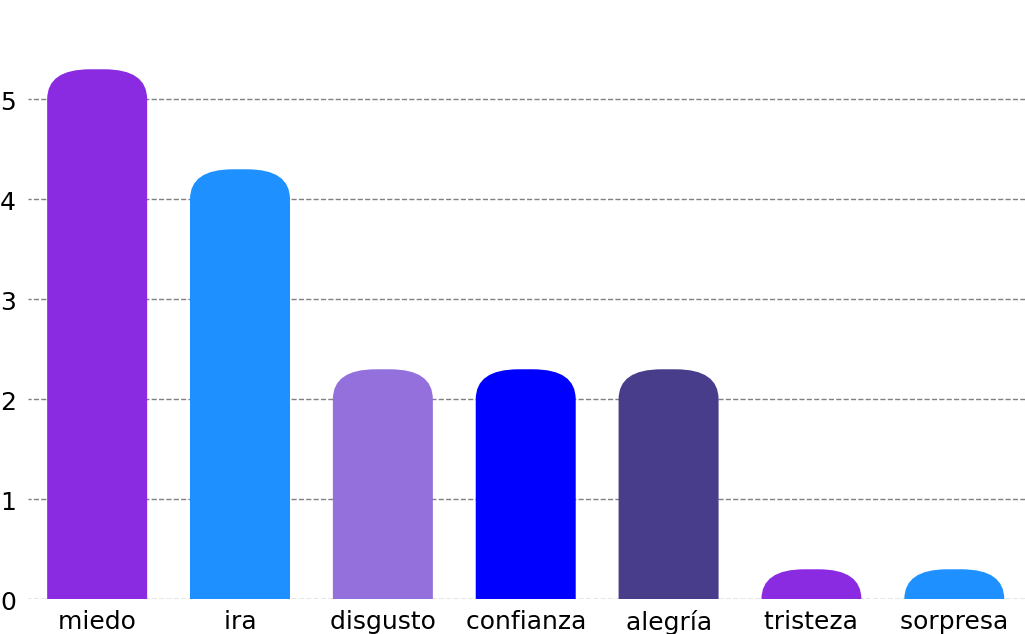
\includegraphics[width=0.8\textwidth]{static/grafica_emociones.png} % Reemplaza con la gráfica de sentimientos
\end{figure}


\begin{figure}[h!]
\begin{flushleft}
    \vspace{1em}
    \marginnote{\scriptsize \parbox{3cm}{\justify En el ámbito del desarrollo organizacional y la ciencia de datos, el análisis de nubes de palabras es una herramienta muy poderosa para comprender las percepciones y actitudes de los colaboradores respecto a las relaciones y procesos que existen dentro de la organización.

    A través de nuestros algoritmos de interpretación semántica entregamos datos y correlaciones de palabras segmentadas de acuerdo a diferentes variables: sexo, edad, rol organizacional, etc. que te permitirán diagnosticar y comprender las percepciones de los diferentes colectivos organizacionales de tu análisis. }}
    \begin{tikzpicture}[baseline=(A.base)]
        % Ovalo personalizado
        \node[draw, color=primary, thick, rounded corners=10pt, minimum width=4cm, minimum height=1.3cm, text centered] (A) 
            {\large \textbf{Análisis de Términos Generales}};
        % Línea que conecta el óvalo con la nota al margen
        \draw[thick, color=primary] (A.east) -- ++(7.5cm, 0);
    \end{tikzpicture}
\end{flushleft}
    \centering
    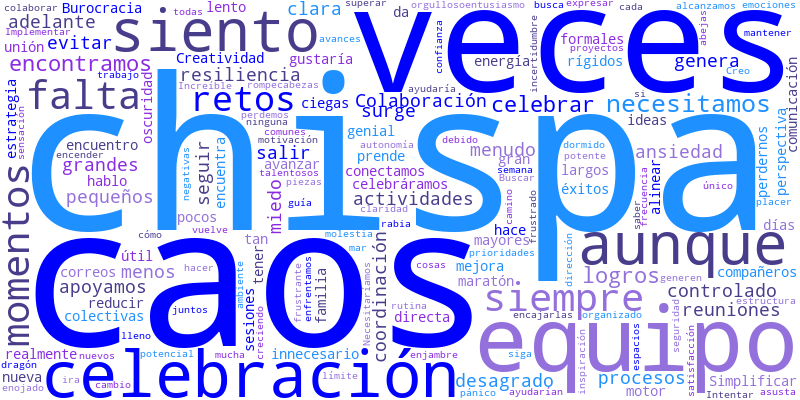
\includegraphics[width=0.8\textwidth]{static/nube_palabras.png} % Reemplaza con la gráfica de sentimientos
\end{figure}
\vskip 2em
\begin{figure}[h!]
    \centering
    \begin{tikzpicture}[baseline=(A.base)]
        % Óvalo personalizado
        \node[draw, color=primary, thick, rounded corners=10pt, minimum width=4cm, minimum height=1.3cm, text centered] (A) 
            {\normalsize \textbf{Análisis de Términos Promotores y Detractores}};
        % Línea que conecta el óvalo con la nota al margen
        \draw[thick, color=white] (A.east) -- ++(7.5cm, 0);
    \end{tikzpicture}
    \vskip 1em
    \begin{minipage}{0.48\textwidth} % Contenedor para Promotores
        \centering
        \begin{minipage}{0.3\textwidth} % Ancho del caption
            \raggedleft
            \begin{tikzpicture}[baseline=(A.base)]
            % Óvalo personalizado
            \node[draw, color=primary, thick, rounded corners=10pt, minimum width=1cm, minimum height=1cm, text centered] (A)
            {\small\textbf{Promotores}};
            \end{tikzpicture}
        \end{minipage}%
        \hspace{2mm}
        \begin{minipage}{0.65\textwidth} % Ancho de la imagen
            
\includegraphics[width=\textwidth]{static/nube_palabras_promotores.png} % Imagen de Promotores
        \end{minipage}
    \end{minipage}%
    \hfill
    \begin{minipage}{0.48\textwidth} % Contenedor para Detractores
        \centering
        \begin{minipage}{0.3\textwidth} % Ancho del caption
            \raggedleft
            \begin{tikzpicture}[baseline=(A.base)]
            % Óvalo personalizado
            \node[draw, color=primary, thick, rounded corners=10pt, minimum width=1cm, minimum height=1cm, text centered] (A)
            {\small\textbf{Detractores}};
            \end{tikzpicture}
        \end{minipage}%
        \hspace{2mm}
        \begin{minipage}{0.65\textwidth} % Ancho de la imagen
            
\includegraphics[width=\textwidth]{static/nube_palabras_detractores.png} % Imagen de Detractores
        \end{minipage}
    \end{minipage}
\end{figure}



\begin{figure}[h!]
    \begin{tikzpicture}[baseline=(A.base)]
        % Óvalo personalizado
        \node[draw, color=primary, thick, rounded corners=10pt, minimum width=4cm, minimum height=1.3cm, text centered] (A) 
            {\normalsize \textbf{Análisis de Términos por Genero}};
        % Línea que conecta el óvalo con la nota al margen
        \draw[thick, color=white] (A.east) -- ++(7.5cm, 0);
    \end{tikzpicture}
    \vskip 2em
    \begin{minipage}{0.5\textwidth}
        \begin{adjustbox}{valign=m}
            \begin{minipage}{2cm} % Contenedor para los textos en vertical
                \begin{tikzpicture}
                    % Primer título "Masculino" en el lado izquierdo de la imagen
                    \node[draw, color=blue, thick, rounded corners=10pt, minimum width=2cm, minimum height=0.8cm, text centered] 
                    {\small \textbf{Masculino}};
                \end{tikzpicture}
                
                \vspace{0.5em} % Espacio entre los textos
                
                \begin{tikzpicture}
                    % Segundo título "Positivo" en el lado izquierdo de la imagen
                    \node[draw, color=blue, thick, rounded corners=10pt, minimum width=2cm, minimum height=0.8cm, text centered] 
                    {\small \textbf{Positivo}};
                \end{tikzpicture}
            \end{minipage}
        \end{adjustbox}
        \begin{adjustbox}{valign=m}
            
\includegraphics[width=10em]{static/nube_palabras_masculino.png} % Reemplaza con tu imagen
        \end{adjustbox}
    \end{minipage}%
    \hfill
    \begin{minipage}{0.5\textwidth}
        \begin{adjustbox}{valign=m}
            \begin{minipage}{2cm}
                \begin{tikzpicture}
                    % Título "Femenino" al lado izquierdo de la imagen
                    \node[draw, color=blue, thick, rounded corners=10pt, minimum width=2cm, minimum height=0.8cm, text centered] 
                    {\small \textbf{Femenino}};
                \end{tikzpicture}
                
                \vspace{0.5em}
                
                \begin{tikzpicture}
                    % Título "Positivo" al lado izquierdo de la imagen
                    \node[draw, color=blue, thick, rounded corners=10pt, minimum width=2cm, minimum height=0.8cm, text centered] 
                    {\small \textbf{Positivo}};
                \end{tikzpicture}
            \end{minipage}
        \end{adjustbox}
        \begin{adjustbox}{valign=m}
            
\includegraphics[width=10em]{static/nube_palabras_femenino.png} % Reemplaza con tu imagen
        \end{adjustbox}
    \end{minipage}
    \hfill

    \vskip 2em
    
    \begin{minipage}{0.5\textwidth}
        \begin{adjustbox}{valign=m}
            \begin{minipage}{2cm} % Contenedor para los textos en vertical
                \begin{tikzpicture}
                    % Primer título "Masculino" en el lado izquierdo de la imagen
                    \node[draw, color=blue, thick, rounded corners=10pt, minimum width=2cm, minimum height=0.8cm, text centered] 
                    {\small \textbf{Masculino}};
                \end{tikzpicture}
                
                \vspace{0.5em} % Espacio entre los textos
                
                \begin{tikzpicture}
                    % Segundo título "Positivo" en el lado izquierdo de la imagen
                    \node[draw, color=blue, thick, rounded corners=10pt, minimum width=2cm, minimum height=0.8cm, text centered] 
                    {\small \textbf{Negativo}};
                \end{tikzpicture}
            \end{minipage}
        \end{adjustbox}
        \begin{adjustbox}{valign=m}
            
\includegraphics[width=10em]{static/nube_palabras_masculino.png} % Reemplaza con tu imagen
        \end{adjustbox}
    \end{minipage}%
    \hfill
    \begin{minipage}{0.5\textwidth}
        \begin{adjustbox}{valign=m}
            \begin{minipage}{2cm}
                \begin{tikzpicture}
                    % Título "Femenino" al lado izquierdo de la imagen
                    \node[draw, color=blue, thick, rounded corners=10pt, minimum width=2cm, minimum height=0.8cm, text centered] 
                    {\small \textbf{Femenino}};
                \end{tikzpicture}
                
                \vspace{0.5em}
                
                \begin{tikzpicture}
                    % Título "Positivo" al lado izquierdo de la imagen
                    \node[draw, color=blue, thick, rounded corners=10pt, minimum width=2cm, minimum height=0.8cm, text centered] 
                    {\small \textbf{Negativo}};
                \end{tikzpicture}
            \end{minipage}
        \end{adjustbox}
        \begin{adjustbox}{valign=m}
            
\includegraphics[width=10em]{static/nube_palabras_femenino.png} % Reemplaza con tu imagen
        \end{adjustbox}
    \end{minipage}
\end{figure}
\end{document}
